\sectioncentered*{Основное содержание}

Во \textbf{введении} делается краткий обзор на область розничной торговли: что из себя представляет, чем занимается, какие основные задачи решает, что можно автоматизировать, какого рода приложения нужны.

\textbf{Первая глава} производит обзор предметной области, а именно уделяется внимание конкретно построению приложений с большими объемами информации. Исходя из самой области применения, бизнес-требования интерпретируются в технические требования, позволяя сформулировать базовые концепты всей системы. Также в этой главе приводится архитектурная модель (схема) стандартных приложений, а также выделяются ее недостатки. В частности, делается вывод о том, что такое приложение быстро превращается в \emph{"клубок"}, который сложно поддерживать и расширять. Вместе с этим дается описание платформы \LB, которую называют еще \emph{smart database} за то, что она в себе содержит все необходимые фукнции, благодаря чему расширяемость приложения не становится больным местом. Среди основных ее идей - сочетание в себе \olap и \oltp технологий, декларативный язык, единая модель модель для бизнес-логики и обработки данных, а также вычислительсные оптимизации, которые хорошо ложатся на данную область. Кроме того, приводится небольшая информация о самой компании \LB, ее структуре, составе, достижениям и тп.

\textbf{Вторая глава} посвящена используемым технологиям. Первая ее часть более подробно раскрывает детали из предыдущей главы, в частности показывается схема самой платформы, делается сравнение \oltp и \olap подходов: когда они применяются, как устроены, какими характеристиками или метриками обладают. Архитектура же базы данных \LB выбрана именно как \emph{общая} (вместо \emph{специализированной}), несмотря на показательные преимущества последней. Успех такого выбора доказывается на примере смартфона, который содержит в себе сторонние функции, кроме мобильной связи.

Далее делается проверка \LB \dbr на соответствие принципам \acid и как они там выражены. Следующий пункт поввящен языку \logiql - центральному компоненту платформы. \logiql является экспрессивным декларативным языком, то есть его легко читать и понимать, а порядок следования инструкций в исходном коде не означает такого же порядка их выполнения, что дарит такую скрытую возможность, как \emph{автоматический параллелизм} выполнения запросов. Также в нем нет пустых значений (\null), используется 6-я нормальная форма, простота в изменении схемы \dbr. Одной из ключевой особенностью является и подход к выполнению операции \join: в случае с попыткой сделать объединение по нескольким предикатам (или таблицам в \sql) платформа \LB пройдется сразу по многим связям, вместо попарных, тем самым позволяя обрабатывать меньший объем данных засчет "отсеивания" по нескольким параметрам сразу. Это достигается с помощью алгоритма \emph{Leapfrom trie-join}, который сводит асимптотику обхода данных в требуемом классе до $O(n\log n)$.

Продолжается описание платформы определением предикатов и этапов выполнения транзакции и как можно с помощью постфиксов \lstinline{@prev}, \lstinline{@initial} и \lstinline{@final} обратиться к данным на этих этапах. Еще приводится немного примеров синтаксиса языка \logiql для агрегаций, правил, ограничений (и как ограничения помогают решать оптимизационные задачи), триггеры и события (они устроены немного по-другому, чем в обычном представлении \sql), запросы и обновления (\emph{queries} и \emph{spreads}). После этого делается переход к самому процессу оптимизации приложений, для чего рассматривается термин \emph{Move computation to data, not vice versa} - дается его толкование, как применяется в платформе и какие выгоды из этого можно получить (к примеру, как на самом деле устроен \emph{автоматический параллелизм}, упомянутый ранее). В завершении дается краткое описание пакетного менеджера \hydra и встроенных веб-сервисов (поскольку они попадают под оптимизацию приложения).

\textbf{Третья глава} рассказывает о цели всей работы - об оптимизации приложения. Из приведенных пояснений о работе платформы делаются заключения по конкретным направлениям, например, исходя из представления данных на диске, операций случайного добавления (размещение по страницам и итерирование по ним по разным ключам). В случае с операцией \join детально разбирается случай с поведением алгоритма в зависимости от порядка ключей, что делает это самым простым, но одним из лучших методов оптимизации. Рассматриваются создание индексов (они создаются автоматически и как при этом расходуются ресурсы по времени и памяти), приводятся рекомендации к пониманию правильных и неправильных (которые лишь усугубят метрики) методов оптимизации. С выбором правильного порядка ключей в предикатах тесно переплетается и другой метод оптимизации - переформулировка правил. Он заключается в том, чтобы содержать правила предельно маленькими по реализации, и разбивать сложные на несколько мелких, логически верных и понятных. Интуиция такого подхода заключается в том, что делать \join
по многим ключам дорого, если при этом нужно обойти несколько придикатов (да еще и, возможно, с разными порядком ключей), поэтому такое "дробление" действительно хорошо сказывается на результатах.

В главе \textbf{Заключение} подытоживаются накопленные советы по оптимизации и приводятся простым перечислением. Также в качестве примера приводятся сравнительные графики работы классических типов запросов в приложении до оптимизации и после. Из них видно, что оптимизация почти не дает выигрыша на мелких запросах, но сравнимо улучшает производительность на сложных запросах и обновлениях. К примеру, приведены два графика с улучшением результатов и без.

\begin{figure}
	\centering
	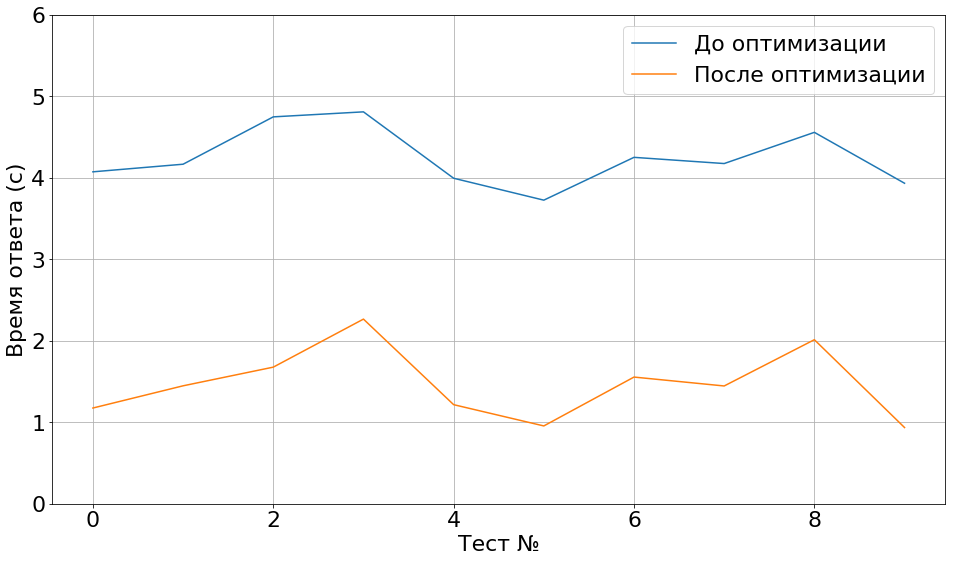
\includegraphics[scale=0.47]{resultByProduct.png}
	\caption{Сравнительный график времени выполнения запроса \lstinline{resultByProduct} до оптимизации и после}
	\label{fig:summary:result_by_product}
\end{figure}

\begin{figure}
	\centering
	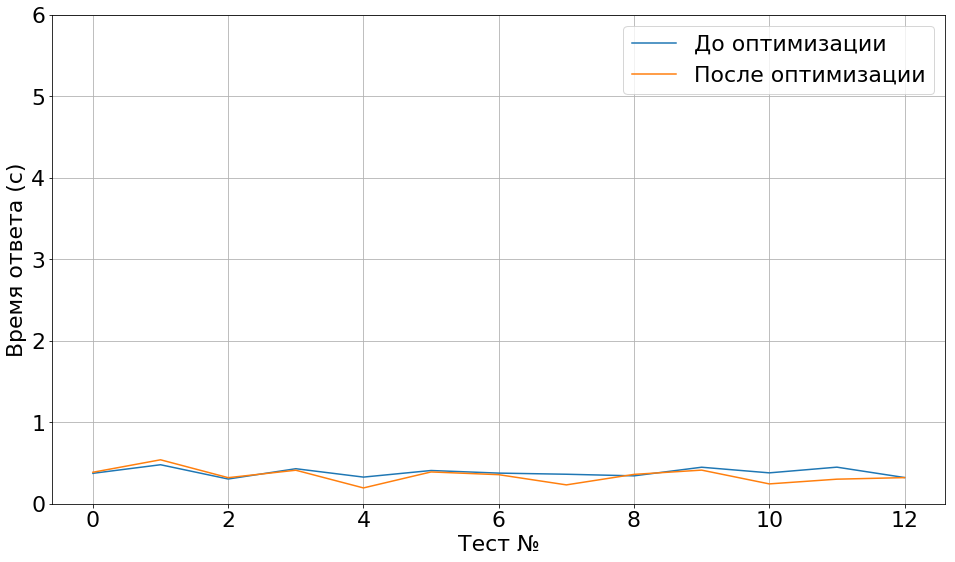
\includegraphics[scale=0.47]{resultByProduct_filtered.png}
	\caption{Сравнительный график времени выполнения запроса упрощенного  \lstinline{resultByProduct} для одного товара до оптимизации и после}
	\label{fig:summary:result_by_product_filtered}
\end{figure}
